%\addcontentsline{toc}{chapter}{Development Process}
\chapter{Design}
\label{section:design}

% \todo[inline]{
% You should concentrate on the more important aspects of the design. It is essential that an overview is presented before going into detail.

% As well as describing the design adopted it must also explain what other designs were considered and why they were rejected.The design should describe what you expected to do, and might also explain areas that you had to revise after some investigation.

% Typically, for an object-oriented design, the discussion will focus on the choice of objects and classes and the allocation of methods to classes. The use made of reusable components should be described and their source referenced. Particularly important decisions concerning data structures usually affect the architecture of a system and so should be described here.How much material you include on detailed design and implementation will depend very much on the nature of the project. It should not be padded out. Think about the significant aspects of your system. For example, describe the design of the user interface if it is a critical aspect of your system, or provide detail about methods and data structures that are not trivial. 

% Do not spend time on long lists of trivial items and repetitive descriptions. If in doubt about what is appropriate, speak to your supervisor. You should also identify any support tools that you used. You should discuss your choice of implementation tools - programming language, compilers, database management system, program development environment, etc. Some example sub-sections may be as follows, but the specific sections are for you to define. 
% }
\section{Hardware}
\begin{figure}
    \centering
    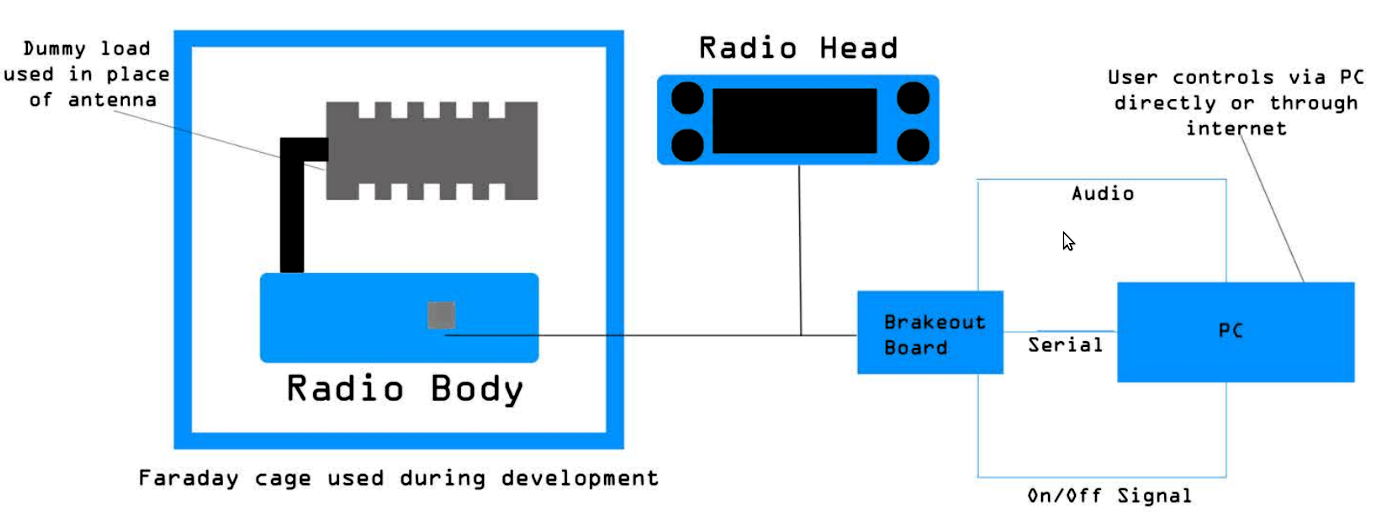
\includegraphics[width=\textwidth]{img/setup_diagram}
    \caption[Hardware Overview]{A hardware overview of the project.}
    \label{fig:setup_diagram}
\end{figure}

\begin{figure}
    \centering
    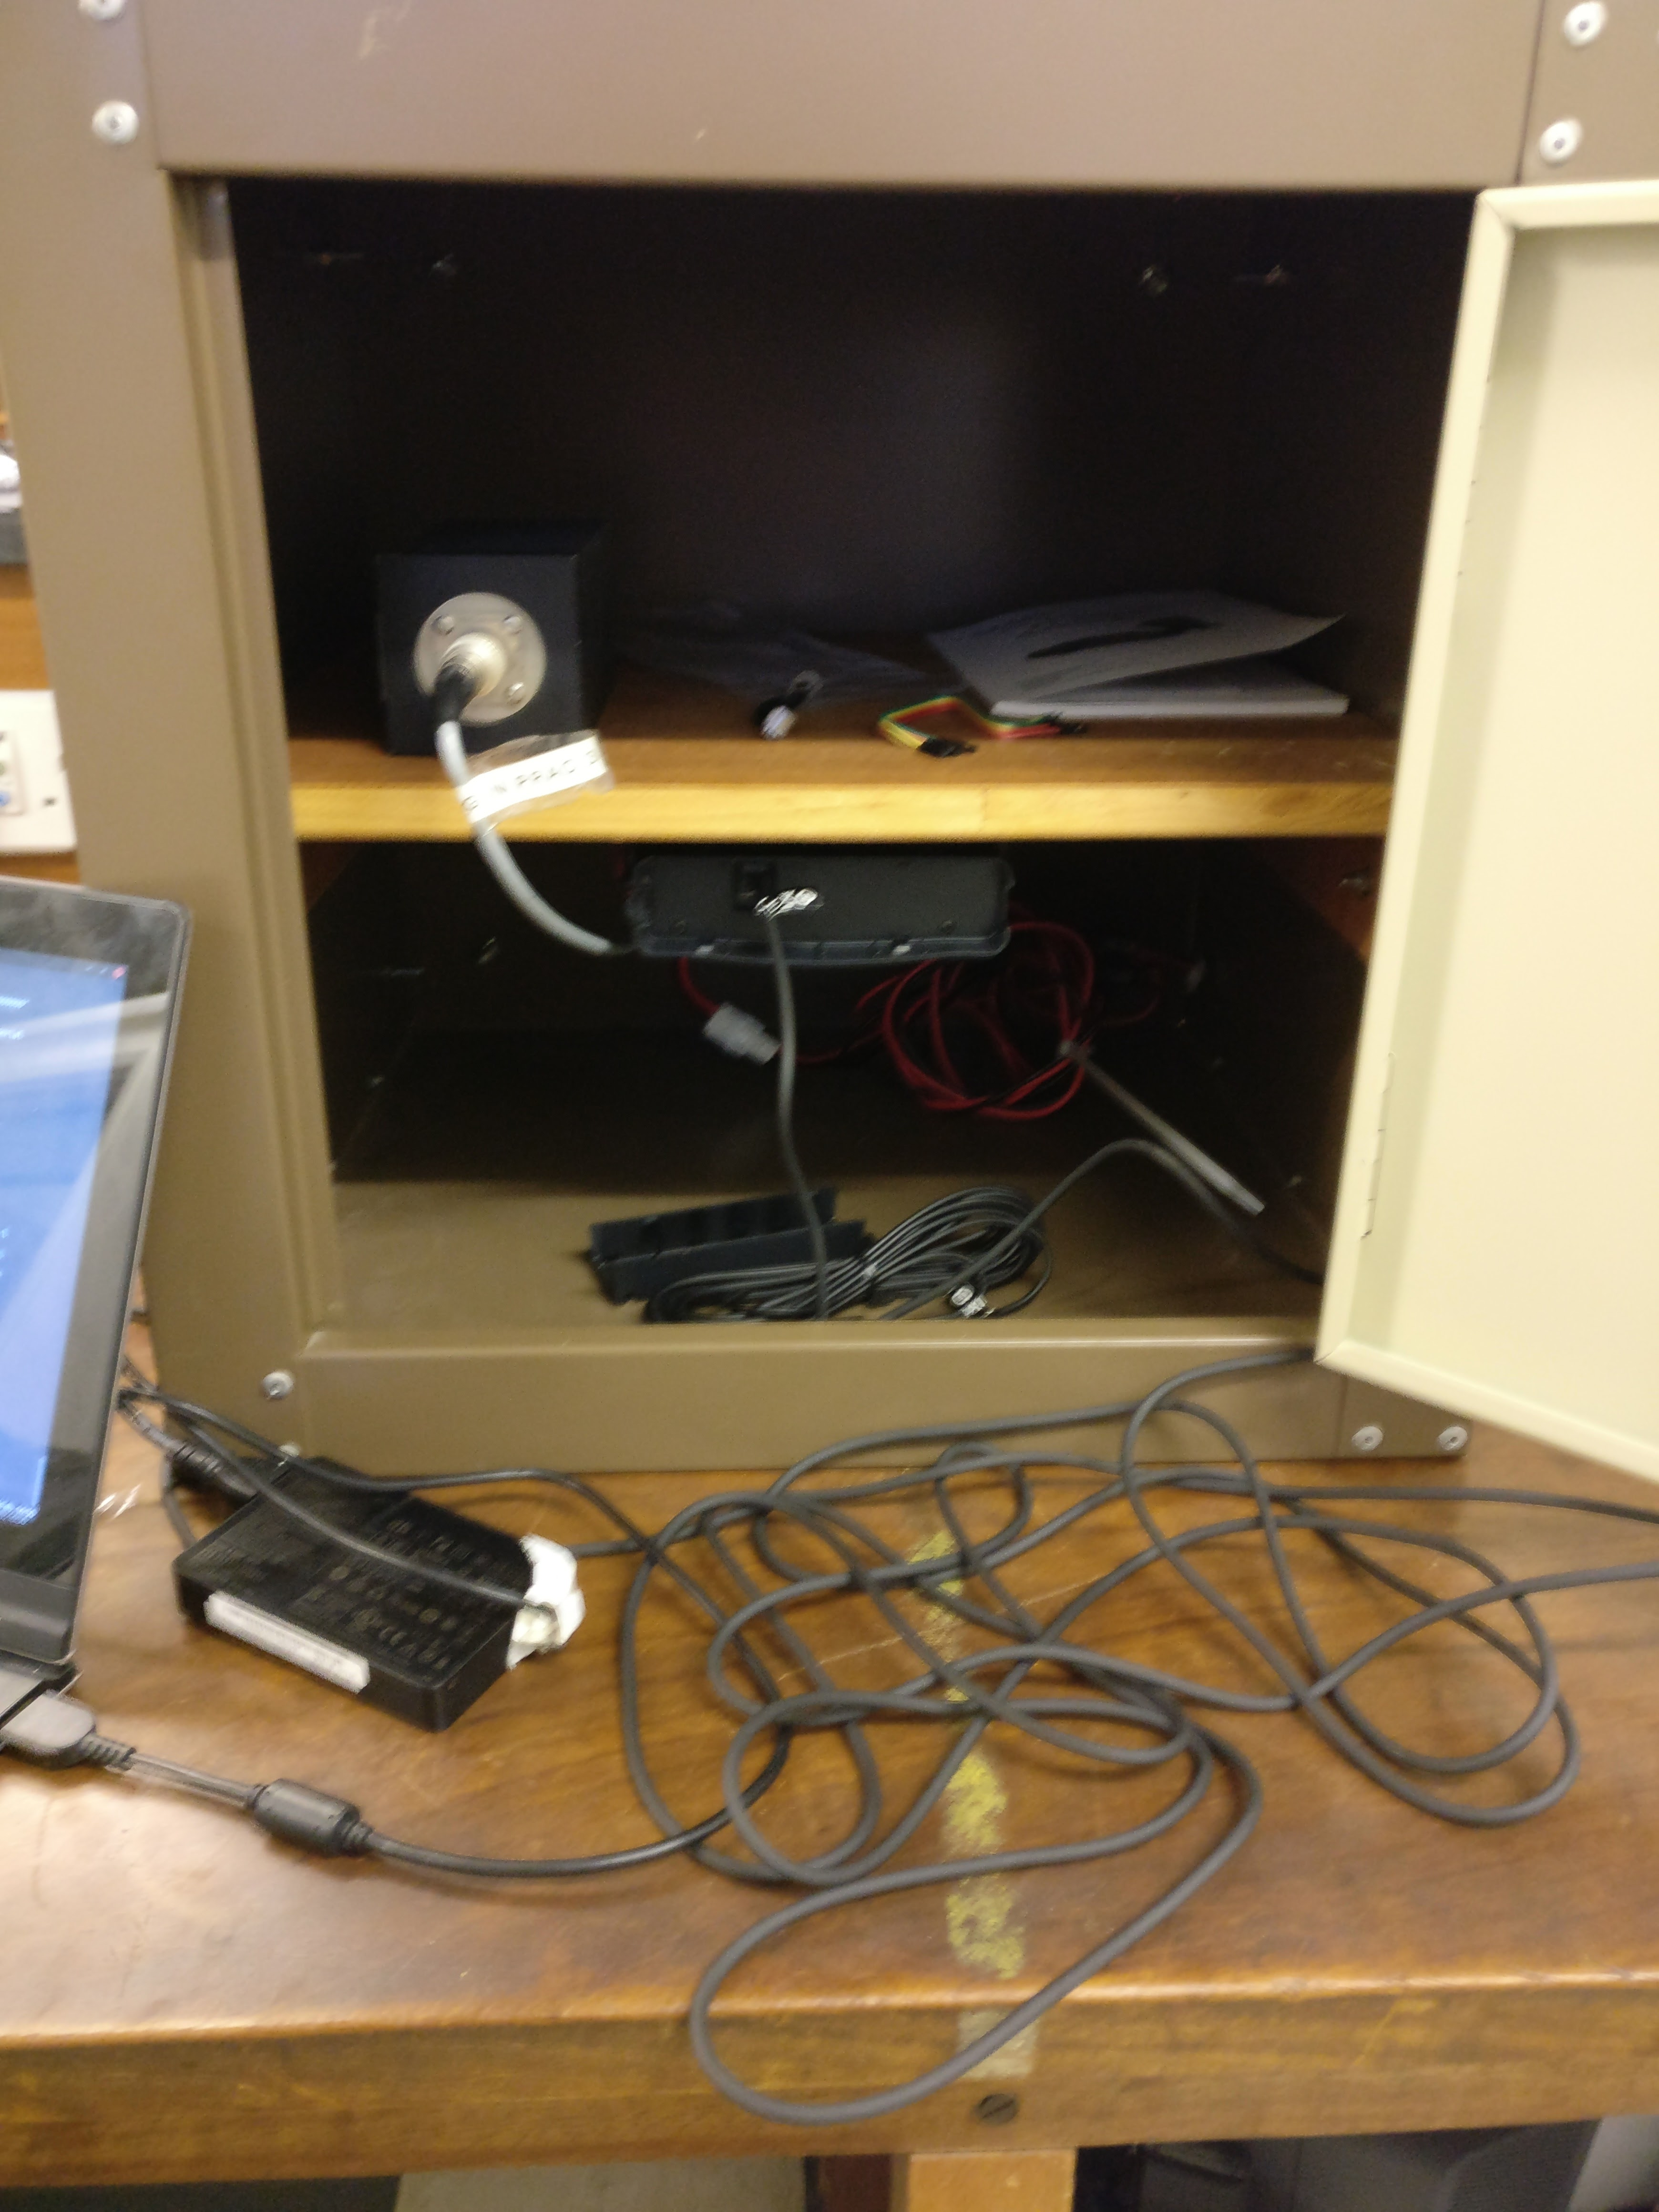
\includegraphics[width=0.5\textwidth]{img/locker.jpg}
    \caption[Radio locker]{A picture of the metal locker used to contain radio waves made from the radio body. The black box below the wooden shelf is the radio body. The box above is the dummy load.}
    \label{fig:locker}
\end{figure}

In order to develop software for the radio, it must be made safe in case of rouge transmissions. To do this the radio was suspended on a wooden shelf placed in a grounded metal locker (See Figure~\ref{fig:locker}). Connected to the radio was a dummy load in place of aerial, with power to the radio coming through a whole in the side of the locker so that the door could remain closed. This helped to reduce the strength of any transmissions significantly but not entirely. As a final precaution a second hand-held radio was placed next to the \gls{8900} to monitor for any transmissions. If this was to occur the developer could then shutdown the radio quickly so as to avoid prolonged transmission.

\begin{figure}
    \centering
    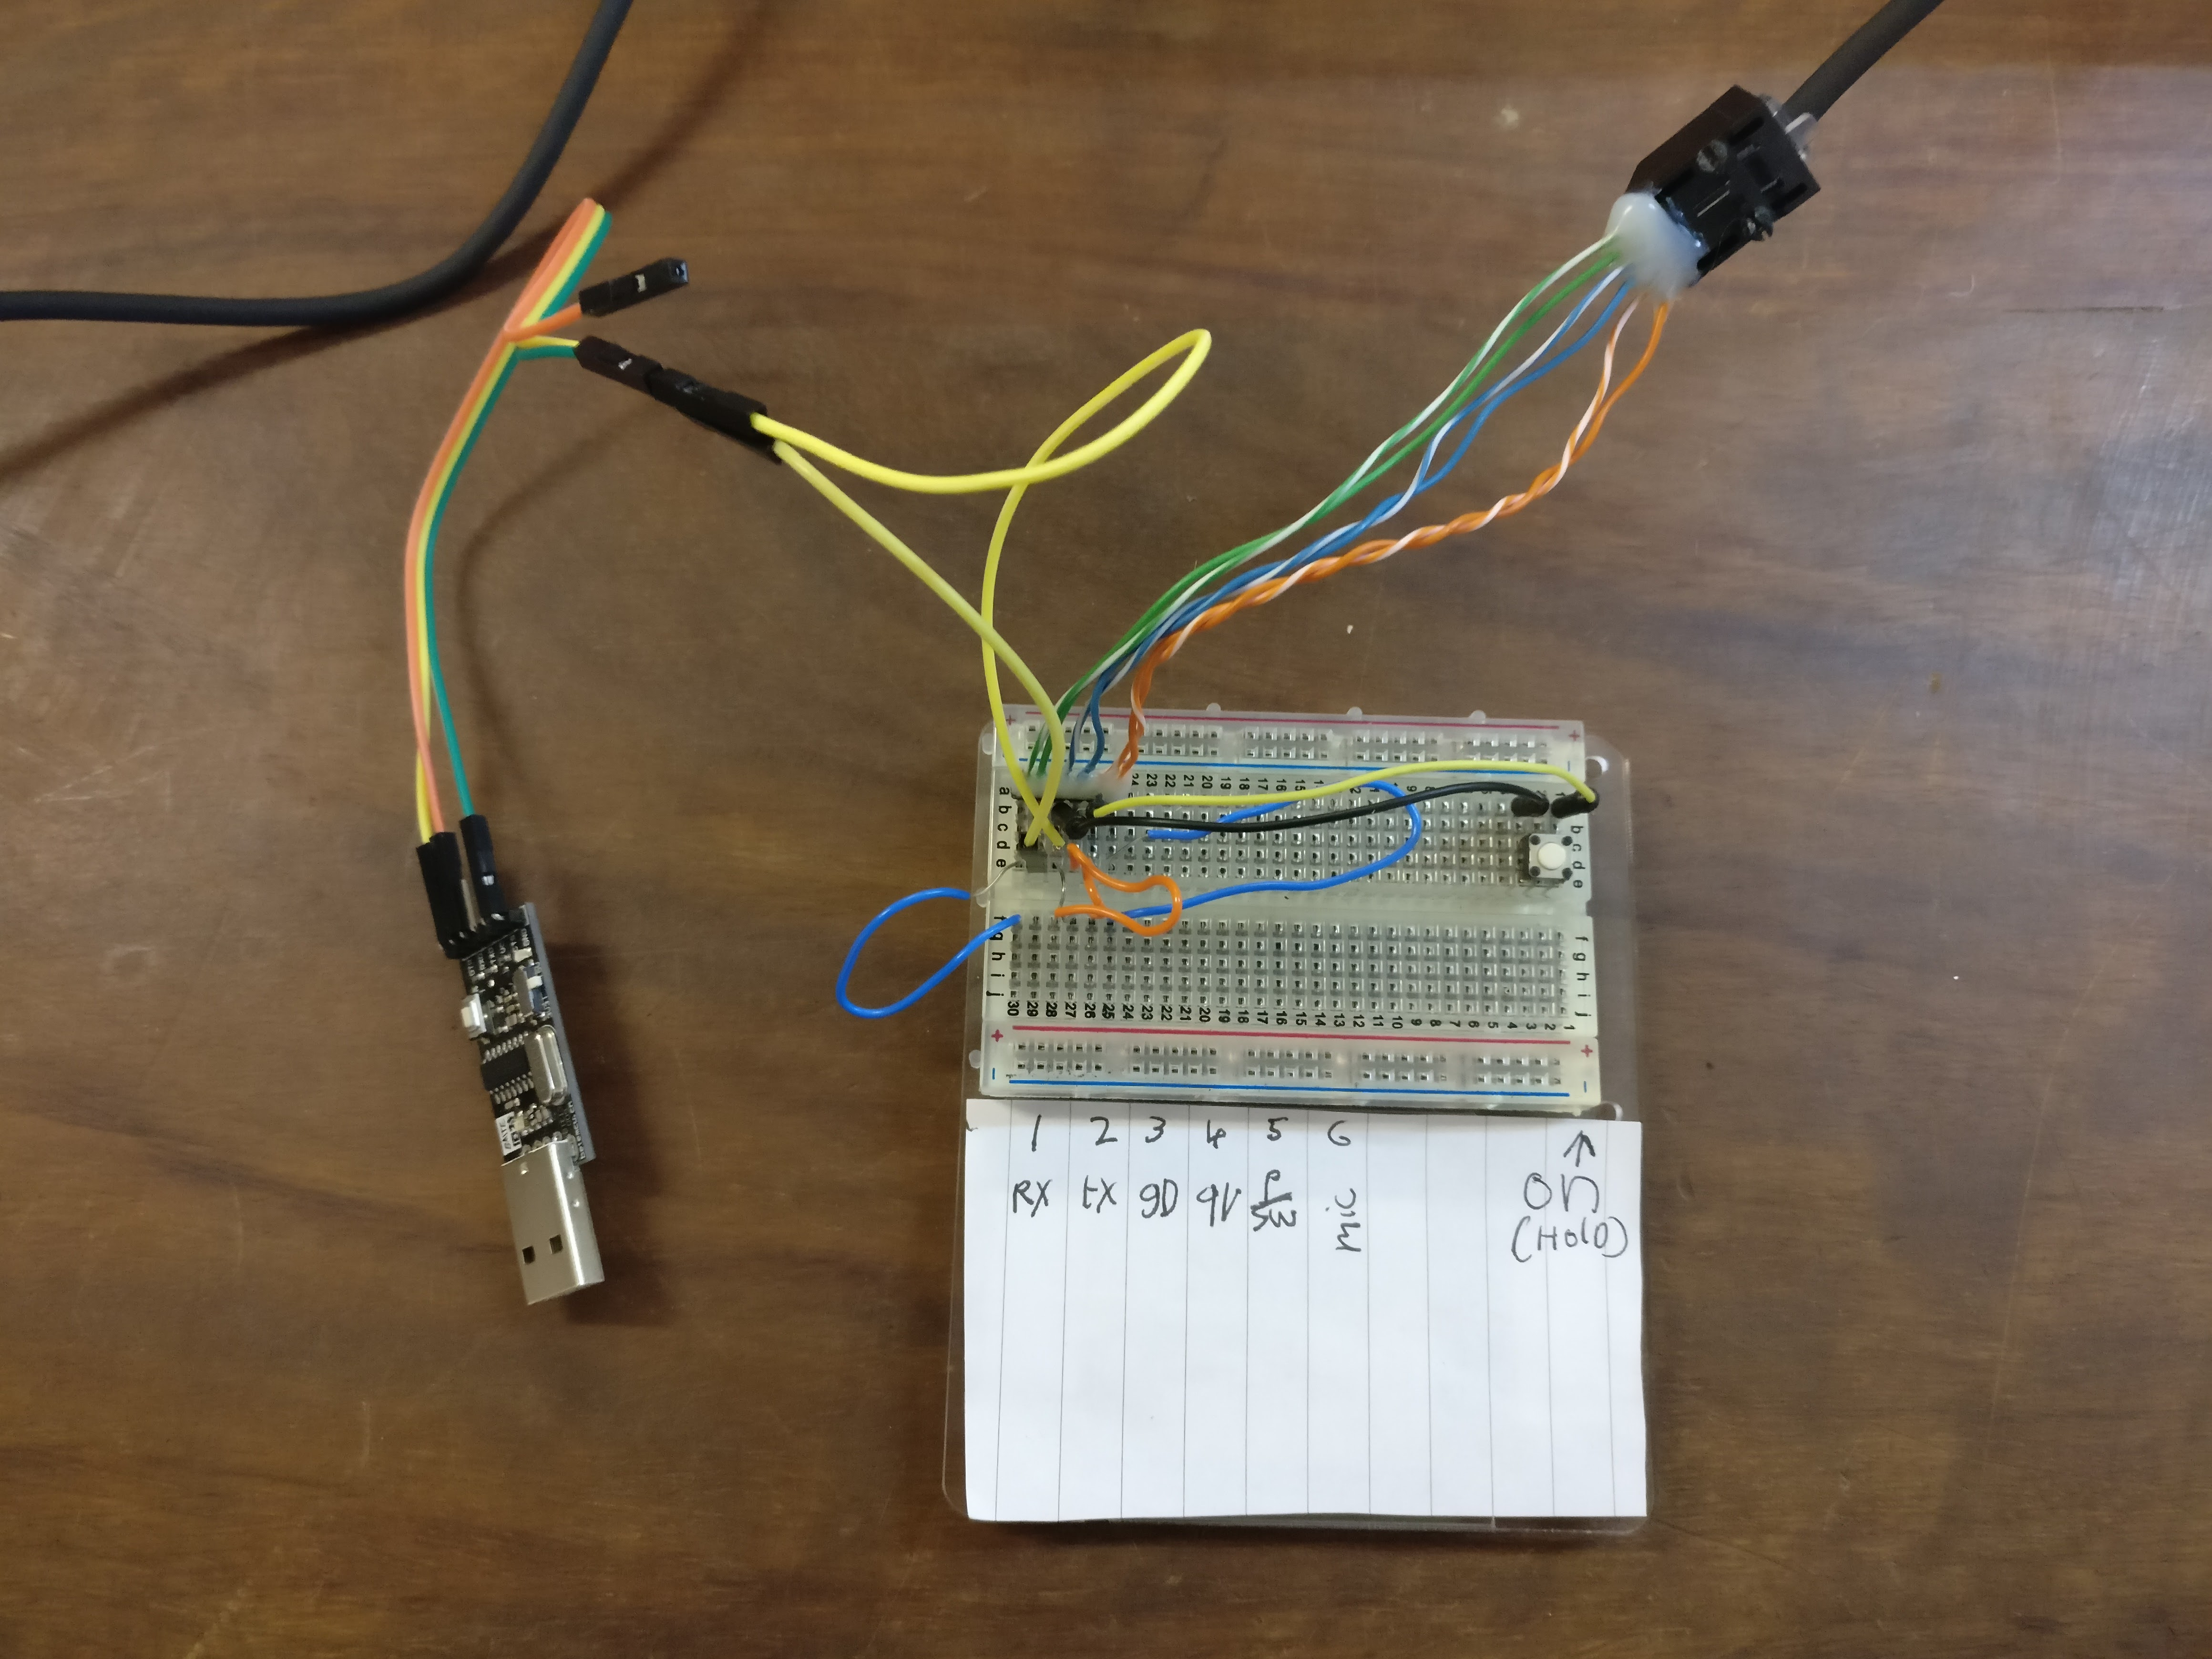
\includegraphics[width=0.9\textwidth]{img/bread_board}
    \caption[Prototype breakout board]{Prototype breakout board used for development.}
    \label{fig:brake_out_board}
\end{figure}

The serial brake-out board (shown in figure~\ref{fig:brake_out_board}) passes though most of the connections to the head of the radio so that the head can still be used. The ground, \gls{rx} and \gls{tx} serial connections are tapped by the serial dongle with the \gls{tx} the only disconnected line from the radio. There is also physical button that connects the power switch to ground when pressed, effectively having the same effect as pressing the power button on the head of the radio.

\section{Overall Architecture}
I will place the more generic functions of the application within a library so that they can be reused in other applications, for example with a different user interface or from a larger application such as Hamlib\cite{hamlib}. My application will provide a console for the user to provide input. I think this is appropriate as the \gls{xp} methodology demands that I keep my design as simple as possible in order to satisfy the acceptance tests. Furthermore as my program is aimed to be in the future an intermediary for signals, not the primary way for the user to control the radio. This is due to the large number of existing and successful free radio control applications designed for such a purpose, for example GRig\cite{grig}. 

\begin{figure}[H]
\centering
    \begin{tikzpicture}[node distance=2cm]
    \node (lib) [process] {libRT8000};
    \node (app) [process, right of=lib, xshift=2cm] {Application};
    \draw [arrow] (lib) -- (app);
    \end{tikzpicture}
    \caption[basic architecture]{The basic overall library/application architecture}
\end{figure}

My design will require that the radio starts receiving a packet every 70ms (50ms to send with 20ms in between). With such a time critical task I will run this routine in a separate thread so that other tasks do not impact on its timing. This is described in figure~\ref{fig:sender_thread}. 

\begin{figure}[ht]
\centering
    \begin{tikzpicture}[node distance=2cm]
% decision, right of=lib, xshift=2cm
    \node (checkq) [decision, xshift=-4cm] {Packet send Queue > 1 ?};
    \node (start) [startstop, above of = checkq, yshift=2cm] {Initialise serial connection, and queue};
        \draw [arrow] (start) -- (checkq);
    
    \node (pop) [process, right of=checkq, xshift=4cm] {Pop and free packet head from memory};
        \draw [arrow] (checkq) -- node[yshift=-0.5cm]{yes}(pop);
        
    \node (peek) [process, below of=pop, yshift=-2cm] {Peek the new head};
        \draw [arrow] (pop) -- (peek);
    
    \node (send) [process, below of=checkq, yshift=-2cm] {Send head packet};
        \draw [arrow] (checkq) -- node[xshift=0.5cm]{No} (send);
        \draw [arrow] (peek) -- (send);
        
    \node (shutdown_q) [decision, left of=send, xshift=-3cm] {Keep alive?};
        \draw [arrow] (send) -- (shutdown_q);
        
    \node (shutdown) [startstop, below of = shutdown_q, yshift=-2cm] {Free remaining queue and return};
        \draw [arrow] (shutdown_q) -- node[xshift=-0.5cm]{No} (shutdown);
        
    \node (wait) [process, left of=checkq, xshift=-3cm] {Sleep 20ms};
        \draw [arrow] (shutdown_q) -- node[xshift=-0.5cm]{Yes} (wait);
        \draw [arrow] (wait) -- (checkq);
    
    \end{tikzpicture}
    \caption[Sender thread]{Flow diagram of the Sender thread}
    \label{fig:sender_thread}
\end{figure}

Items in the queue are only removed (popped) when there is more than a single packet inside. This is because the radio requires constant packets else it will shutdown. To stop this the last packet is resent continuously. Most functions will append to this packet queue to perform an action.

While designing the packet sender thread I came up with the idea of the ``default packet''. This packet contains the constant state of the radio. To change the volume the default packet is directly modified. More complex actions, for example ones that require a button be pressed only momentarily will add new packets to the queue, based on this default packet. As there will possibly be duplicate packets in the queue, the queue implementation must hold only a references to the default packet.

I is anticipated that the bulk of memory usage will be to store representations of packets. Therefore the data structure should be as memory efficient as possible. Although this must balance with the ease of use i.e sections being able to be mapped accordingly. I will store the packet as a bitfield so that the \gls{rx} packet will take up only 42 bytes (or as close to this as possible). I will then use bit-wise operations to read and set bits inside the packet. This has the added benefit that sending via serial will not require any additional processing, as the representation is identical.

Packets sent to the screen (\gls{rx}) will hereby be referred to as ``display packets''. These they are used to generate the output of the display, where a set bit in the packet corresponds to an illuminated segment on the display. The packets that are \gls{tx} to the radio body will be referred to ``control packets'' as they communicate the current state of the controls back to the radio.

\begin{figure}[H]
\centering
    \begin{tikzpicture}[node distance=2cm]
    \node (app) [process] {Application};
    \node (lib) [process, below of=app] {libRT8000};
        \draw [arrow] (app) -- (lib);
        \node (control) [process, below of=lib, xshift=-2cm] {Control Packet};
        \node (disp) [process, below of=lib, xshift=2cm] {Display Packet};
        \draw [arrow] (lib) -- (control);
        \draw [arrow] (lib) -- (disp);
            \node (packet) [process, below of=disp, xshift=-2cm] {packet};
             \draw [arrow] (control) -- (packet);
             \draw [arrow] (disp) -- (packet);
    \end{tikzpicture}
    \caption[Overall architecture]{A more detailed vision of relations of the application}
    \label{overall_architecture}
\end{figure}

\section{Language choice}
\label{section:language_choice}

I chose a number of candidate languages that I believe may be appropriate. To decide on what to use I have set out five main criteria: 
\begin{itemize}
    \item Prior experience
    \item Existing serial support
    \item Ease of bitfield storage
    \item Portability
    \item Speed
\end{itemize}

\section*{Python}
Python is the language I have the most experience in using. First I created a scratch program to show that is was actually possible to store Bitfields and map the relevant sections to it (See section \ref{python_bitfield} for this code). This proved promising but I wanted to know how compact this was in memory. To do this I created a 336 bit number (42 bytes) and queried how much space the interpreter has allocated for it. 

\begin{minted}{python}
>>>import sys

>>>a = (1 << 336)
>>>sys.getsizeof(a)
72
\end{minted}

Python has given a 71\% overhead to our bitfield. 30 bytes more than needed is sub-optimal for our usage.

My other concern was how fast the serial library was in Python. While Python does not have serial in its standard library, it does has a well supported third party library named ``PySerial''\cite{pyserial}. I wrote a scratch program to test this.

\begin{minted}{python}
import serial
ser = serial.Serial('/dev/ttyUSB0')  # open serial port

for _ in range(100):
    ser.write((1 << 336))
    ser.flush() # wait until message sent

ser.close()  
\end{minted}

This program sends 100 x 336 bits as fast as possible to the serial device located named ``ttyUSB0''. I then connected the serial line to a digital oscilloscope to measure the performance. The width between packets was a high 40ms, where the actual delay of the radio was 20ms between packets.

While at the time I found this unacceptable it turns out that the body of the radio could tolerate up to and past 50ms of delay \todo[]{put upper bound here}. However I think I made the right choice as these performance issues could have become a problem further into development. In addition a lower level language would give me the opportunity for an application with less resource usage.

\section*{Golang}
Golang is a new compiled language created in 2007. It brings lots of the newer ideas that interpreted languages have used such as type inheritance and method overloading. Golang was designed supplant the C programming language. One of the original authors of Golang is Ken Thompson (who is also one of the original authors of C). Its syntax is a combination of C and python, yet it is more strict than either, for example including an unused import will throw a compiler error and  having a definitive style guide instead of competing standards.

Golang could be the ideal language to use in the future, but currently its standard library does not support serial communication. The most supported third party library is still in the alpha stage. This ruled out Golang over competing languages that already had a stable \gls{api} for such actions.

\section*{C}
Other projects of similar nature have used C (including other ham radio drivers). C allows you to define a data structure with an very exact number of bytes.

\begin{minted}[breaklines]{c}
//adapted from http://stackoverflow.com/questions/8584577/access-bits-in-a-char-in-c

//This tells the compiler to not put padding bits between values in the struct.
#pragma pack(1) //as we don't want space between our bits here
typedef struct {
        unsigned int data: 7;      // 7 more bits of the byte
        unsigned int check_num: 1; // Used to signify the first byte in the packet
} FT8900BYTE;

typedef union { 
        FT8900BYTE section;
        unsigned char raw;
} PACKET_BYTE;
#pragma pack()

int main()
{
        PACKET_BYTE packet[42];
        return 0;
}
\end{minted}

C also has serial support in its standard library with the include``<termios.h>''. While this is not as simple to use as other languages, it is the most comprehensive of them by far. Although ``Pyserial'' may have had a had better timeout implementation as it had a hard limit of seconds after the last bit instead of time between packets like the C implementation.

\section*{Comparison}
Table~\ref{table:language_comparison} summarises my comparison of candidate languages. Despite my lack of experience, C won out by 11 points. When working in C, a quick check of how much involvement of strings there will be is necessary, as strings are a weakness of the language. I concluded that only the logging and shell will involve heavy use of strings, meaning that the bulk of my code would not be affected.

\begin{table}[h!]
\centering
\begin{tabular}{|l| c c c c c |c|} 
 \hline
 Language & experience & serial support & bitfield storage & portability & speed & total\\
 \hline\hline
  Python & 9 & 5 & 5 & 6 & 4 & 29 \\
 \hline
 Golang  & 4 &  2 &  8 &  7 & 10 & 31\\
 \hline
 C       & 2 & 10 & 10 & 10 & 10 & 42\\
\hline
\end{tabular}
\caption{Summary of languages comparison}
\label{table:language_comparison}
\end{table}


